\documentclass[10pt,letterpaper]{article}
\usepackage{graphicx}
\usepackage[margin=0.8in]{geometry}
\pagestyle{empty}

\begin{document}
\centerline{\Large \bf replicate-1, mutvir\_MS}
\vspace{0.3in}

\center{\begin{minipage}{4.3in}
\centerline{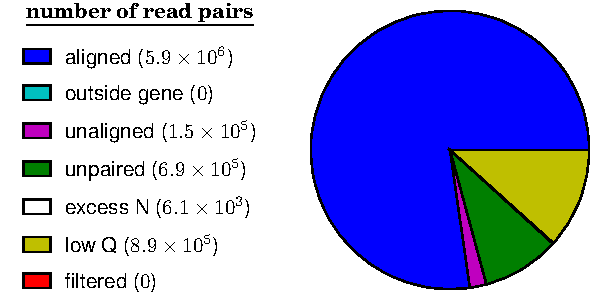
\includegraphics[width=4in]{replicate-1-mutvir_MS_alignmentstatistics.pdf}}
\vspace{0.3in}

\centerline{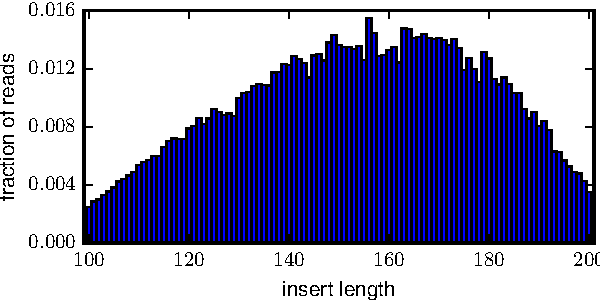
\includegraphics[width=4in]{replicate-1-mutvir_MS_insertlengths.pdf}}
\end{minipage}
\begin{minipage}{2.1in}

\underline{\large \bf Alignment settings}
\begin{description}
\item[minq = 25.0]
Both reads must have mean Q-value $\ge$ this.
\item[maxn = 5]
Number of N/n nucleotides must be $\le$ this for each read.
\item[minoverlap = 100]
Overlap between paired reads must be $\ge$ this.
\item[maxrm = 1]
Number of mismatches in paired reads overlap must be $\le$ this.
\item[maxa1m = 1]
Number of mismatches between R1 and its adaptor must be $\le$ this.
\item[maxa2m = 1]
Number of mismatches between R2 and its adaptor must be $\le$ this.
\item[maxgenem = 10]
Neither read can have $>$ than this many mismatches with target sequence after trimming adaptor.
\end{description}
\end{minipage}}
\vspace{0.3in}

\centerline{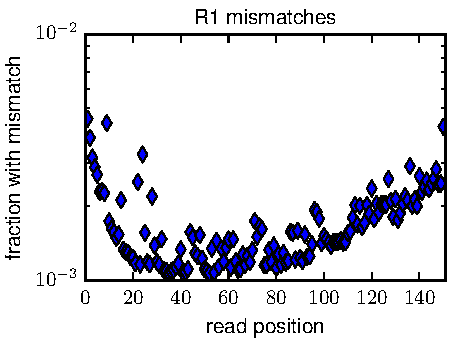
\includegraphics[width=3in]{replicate-1-mutvir_MS_R1mismatches.pdf}\hspace{0.3in}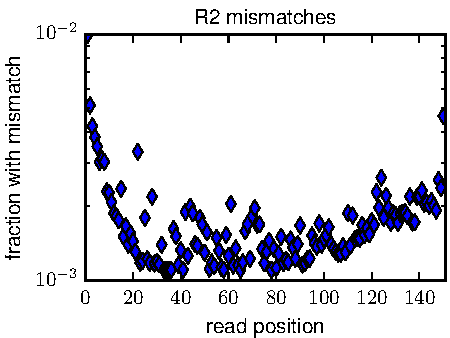
\includegraphics[width=3in]{replicate-1-mutvir_MS_R2mismatches.pdf}}
\end{document}
